\section{Kreuz-Prädiktion}
\label{sec:exp_cross_pred}
Momentan ist es durch invitro Experimente bereits möglich die Ausbreitung der elektrischen Erregung auf der Oberfläche des Herzmuskels experimentell aufzuzeichnen. Nun stellt sich die Frage, ob anhand beispielsweise der Messung der Membramspannung weitere Variablen des Systems wie die Kalium-Konzentration oder ähnliches ermittelt werden kann. Diese Fragestellung wird in der ersten Aufgabe betrachtet. Es wird die Vorhersage von der Spannungsvariable auf die zweite Variable des jeweiligen Modells sowohl für das \textit{Barkley}- als auch für das \textit{Mitchell-Schaeffer}-Modell durchgeführt. Dabei wird zuerst die Nächste Nachbar Methode, anschließend die radialen Basisfunktionen und schlussendlich die \textit{ESN}s verwendet. Es werden sowohl die einzelnen Ergebnisse präsentiert als auch ein abschließender Vergleich durchgeführt.
 
\subsection{Nächste Nachbar Vorhersage}
Die Ergebnisse für die optimalen Hyperparameter des Modells $\delta \in \{3,4,5\}, k \in \{2, 3, 4, 5\}$ sind in Tabelle \ref{tab:exp_cross_nn_results} zu finden. Die Werte für $\sigma$ und $\Delta \sigma$ sind wie zuvor beschrieben variiert worden. Dabei sind sowohl die verwendeten Parameter als auch die erzielten Fehler MSE und NRMSE aufgelistet.
\begin{table}[h]
	\centering

	\begin{tabular}{ccc}
		\hline		
		\multicolumn{1}{c}{} & Barkley & Mitchell-Schaeffer \\ 
		\hline 
		\rule[-1ex]{0pt}{2.5ex} $\sigma$ & $1$ & $7$ \\ 
		\rule[-1ex]{0pt}{2.5ex} $\Delta \sigma$ & $1$ & $1$ \\ 
		\rule[-1ex]{0pt}{2.5ex} $\delta$ & $3$ & $3$ \\ 
		\rule[-1ex]{0pt}{2.5ex} k & $5$ & $5$ \\ 
		\rule[-1ex]{0pt}{2.5ex} Laufzeit [s] & $40$ & $5252$ \\ 
		\rule[-1ex]{0pt}{2.5ex} \textbf{MSE} & \textbf{0.00098} & \textbf{0.01891} \\ 
		\rule[-1ex]{0pt}{2.5ex} \textbf{NRMSE} & \textbf{0.1317} & \textbf{0.8795} \\ 
		\hline 
	\end{tabular} 

	\caption{Ermittelte Hyperparameter der nächsten Nachbar Vorhersage für das \textit{Mitchell-Schaeffer}- und das \textit{Barkley}-Modell, welche zu den geringsten Fehlern führen.}
\label{tab:exp_cross_nn_results}
\end{table} 

Dabei ist die stark unterschiedliche Laufzeit der beiden Vorhersagen auffällig. Dies lässt sich allerdings durch die verschiedenen Dimensionalitäten der Quellvariable erklären: Während beim \textit{Barkley}-Modell lediglich ein $3$-dimensionaler Vektor für die Vorhersage die besten Ergebnisse erzielt konnte beim \textit{Mitchell-Schaeffer}-Modell durch die Verwendung eines $147$-dimensionalen Quellvektors die besten Ergebnisse erzielt werden. Da, wie in Abschnitt \ref{sc:theory_nn} erwähnt, die benötigte Zeit für eine Vorhersage sehr stark mit der Dimension zunimmt, lässt sich somit der Anstieg von $40$ auf $5252$ Sekunden erklären.

Da eine Nächsten Nachbar Vorhersage nur anhand der in der Trainingsphase gesehenen Datenpunkte eine Vorhersage erstellt, ist anzunehmen, dass die Qualität dieser sehr stark von der Länge der Trainingsphase abhängt. Um dies zu untersuchen ist für die zuvor ermittelten Hyperparameter eine Vorhersage für verschiedene Trainingslängen $N_{Training}$ durchgeführt und die dabei auftretenden MSEs und die benötigte Laufzeit gemessen worden. Hierbei können zwei Effekte beobachtet werden. Bei der Betrachtung der grafischen Darstellung der benötigten Laufzeit in Abbildung \ref{fig:exp_cross_nn_trainlength_mse_time_barkley} für das \textit{Barkley}-Modell ist zu erkennen, dass sich der Zusammenhang zwischen $N_{Training}$ und der Laufzeit durch eine logarithmische Ausgleichskurve beschreiben lässt. Dies ist nach der theoretischen Betrachtung in \ref{sc:theory_nn} ein erwartetes Ergebnis. Der erzielte Fehler verhält sich dagegen anders und sinkt asymptotisch gegen eine untere Schranke ab. 

\begin{figure}[H]
	\centering
	\begin{subfigure}{.95\textwidth}
		\centering
		\hspace*{0.3cm}
		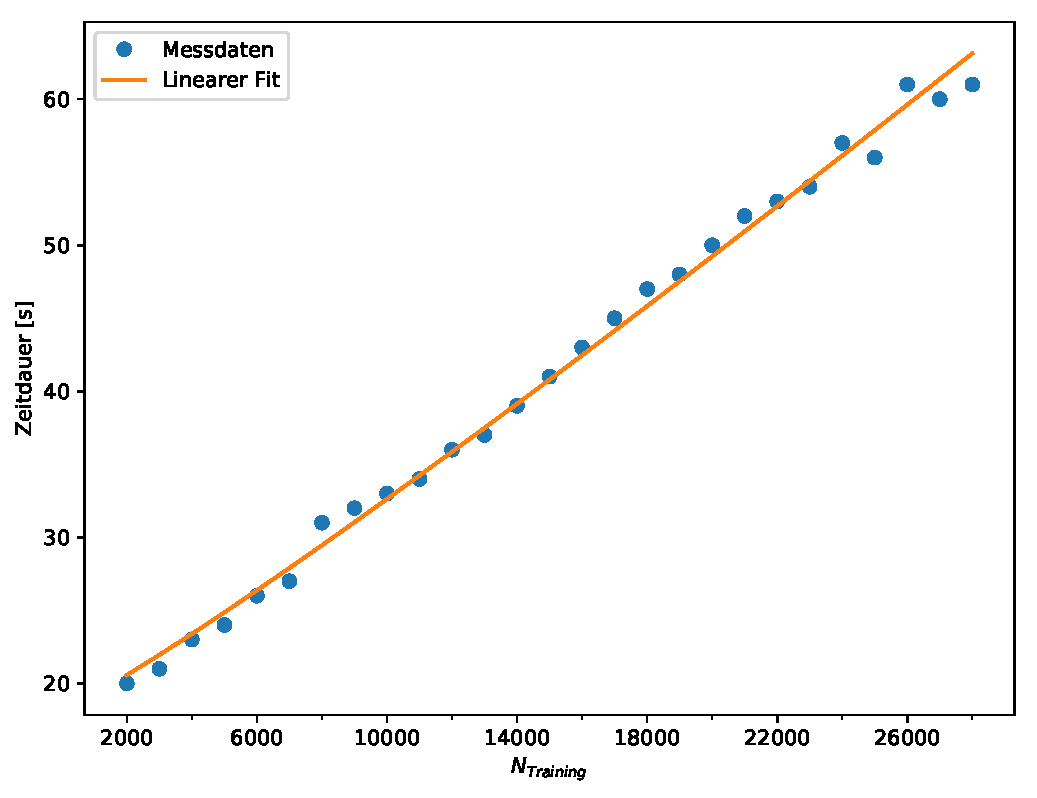
\includegraphics[width=.76\textwidth]{figures/results/cross_prediction/nn_trainlength_uv_time.pdf}
		\caption{Abhängigkeit der Laufzeit von $N_{Training}$.}
	\end{subfigure}%
	\\
	\begin{subfigure}{.95\textwidth}
		\centering
		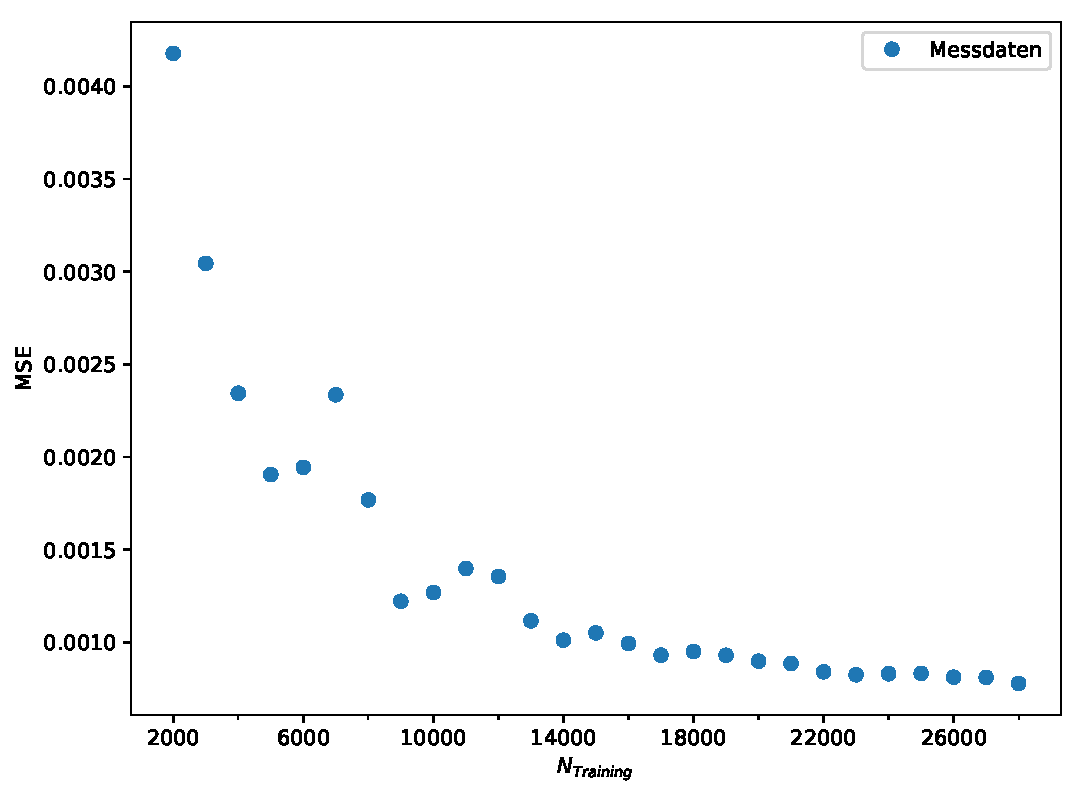
\includegraphics[width=.80\textwidth]{figures/results/cross_prediction/nn_trainlength_uv_mse.pdf}
		\caption{Abhängigkeit des \textit{MSE}s von $N_{Training}$.}
	\end{subfigure}%
	\caption{Darstellung der Abhängigkeit des benötigten Laufzeit (oben) und des MSE (unten) von der verwendeten Anzahl an Trainingsdaten $N_{Training}$ (unten) für das \textit{Barkley}-Modell bei der Verwendung einer nächsten Nachbar Vorhersage.}
	\label{fig:exp_cross_nn_trainlength_mse_time_barkley}
\end{figure}

Eine Analoge Darstellung für das \textit{Mitchell-Schaeffer}-Modell ist in \ref{fig:apx_exp_cross_nn_trainlength_mse_time_ms} zu finden. Anzumerken ist, dass die Sättigung des Fehlers im \textit{Barkley}-Modell schon ab etwa $N_{Training}=15000$ eintritt, doch beim \textit{Mitchell-Schaeffer}-Modell erst deutlich später. Dies ist ein Hinweis darauf, dass die Dynamiken im letzteren chaotischer und unregelmäßiger als bei ersten ablaufen. Zusammenfassend lässt sich somit die Wahl der Trainingslänge von $N_{Training} = 15000$ für alle Szenarien und alle drei Methoden damit begründen, dass man für die Nächste Nachbar Vorhersage, welche am empfindlichsten auf diese Länge reagiert, eine akzeptablen Kompromiss zwischen der Rechenzeit und der Genauigkeit erhält.

\FloatBarrier
\subsection{Radiale Basisfunktionen}
Bei der Verwendung radialer Basisfunktionen stellt zudem die Breite $\sigma_{RBF}$ der Gaußfunktionen als auch die Anzahl der Basisfunktionen $l$ einen wichtigen Parameter dar. Im Rahmen dieser Arbeit ist die Anzahl der Basisfunktionen auf $l=100$ festgelegt worden - diese Wahl wird im Folgenden weiter motiviert werden. Um die anderen Parameter zu finden, sind $\sigma$, $\Delta \sigma$ wie oben beschrieben, $\delta \in \{3,4,5\}$ und $\sigma_{RBF} \in \{0.5, 1.0, 3.0, 5.0, 7.0, 9.0\}$ variiert worden. In Tabelle \ref{tab:exp_cross_rbf_results} sind die dadurch gefundenen optimalen Parameter, die damit erreichten Fehler und die benötigte Laufzeit erneut für beide Modelle aufgelistet. Hierbei ist zu bemerken, dass die optimalen Werte für $\sigma$, $\Delta \sigma$ und $\delta$ mit denen für die NN-Vorhersage übereinstimmen. 

\begin{table}[h]
	\centering

	\begin{tabular}{ccc}
		\hline 			
		\multicolumn{1}{c}{} & Barkley & Mitchell-Schaeffer \\ 
		\hline 
		\rule[-1ex]{0pt}{2.5ex} $\sigma$ & $1$ & $7$ \\ 
		\rule[-1ex]{0pt}{2.5ex} $\Delta \sigma$ & $1$ & $1$ \\ 
		\rule[-1ex]{0pt}{2.5ex} $\delta$ & $3$ & $3$ \\ 
		\rule[-1ex]{0pt}{2.5ex} $\sigma_{RBF}$ & $0.5$ & $5$ \\ 
		\rule[-1ex]{0pt}{2.5ex} Laufzeit [s] & $1430$ & $1434$ \\ 
		\rule[-1ex]{0pt}{2.5ex} \textbf{MSE} & \textbf{0.01046} & \textbf{0.00948} \\ 
		\rule[-1ex]{0pt}{2.5ex} \textbf{NRMSE} & \textbf{0.1023} & \textbf{0.6228} \\ 
		\hline 
	\end{tabular} 
	\caption{Ermittelte Hyperparameter der radialen Basisfunktionen für das \textit{Mitchell-Schaeffer}- und das \textit{Barkley}-Modell, welche zu den geringsten Fehlern führen.}
	\label{tab:exp_cross_rbf_results}
\end{table} 

Analog zu der Untersuchung des Einflusses der Trainingslänge $N_{Training}$ bietet es sich für die radialen Basisfunktionen an, den Einfluss der Anzahl der verwendeten Basisfunktionen $l$ auf die Genauigkeit und die benötigte Laufzeit zu untersuchen, um die zuvor angegebene Wahl $l=100$ zu begründen. Dabei werden jeweils wieder die besten zuvor ermittelten Hyperparameter verwendet. Hierfür sind die gemessenen Laufzeiten gegen die Anzahl der Basisfunktionen $l$ in Abbildung \ref{fig:exp_cross_rbf_placements_time_barkley} für das \textit{Barkley}-Modell aufgetragen worden. Zusätzlich ist auch der Zusammenhang zwischen dem erreichten MSE und der Anzahl der Basisfunktionen in Abbildung \ref{fig:exp_cross_rbf_placements_mse_barkley} aufgetragen. Eine dazu analoge Darstellung für das \textit{Mitchell-Schaeffer}-Modell ist in Abbildung \ref{fig:apx_exp_cross_rbf_placements_time_mse_ms} zu finden. Es ist erneut anzunehmen, dass näherungsweise ein linearer Zusammenhang zwischen der Laufzeit und der Anzahl der Basisfunktionen auf dem untersuchten Bereich besteht.

\begin{figure}[h]
	\centering
	\begin{subfigure}{\textwidth}
		\centering
		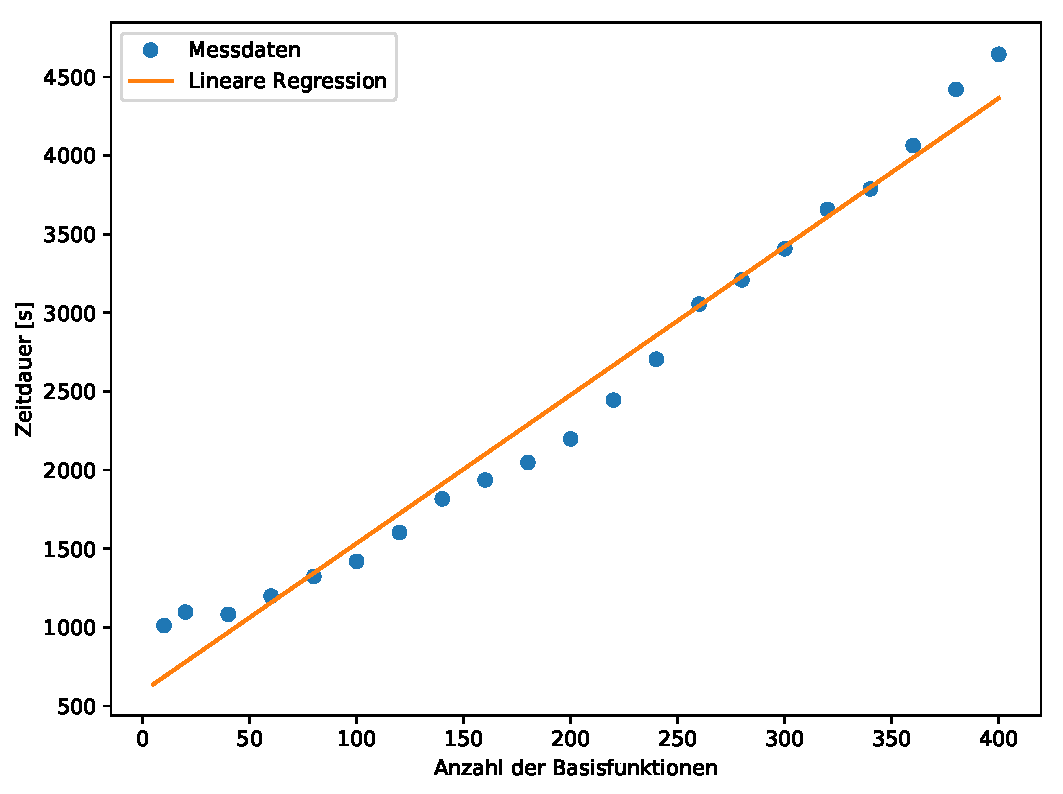
\includegraphics[width=4.2in]{figures/results/cross_prediction/rbf_placements_uv_time.pdf}
		\caption{Abhängigkeit der Laufzeit von $l$.}
	\end{subfigure}%
	\caption{Darstellung der Abhängigkeit des benötigten Laufzeit von der Anzahl der Basisfunktionen $l$ für das \textit{Barkley}-Modell\textit{Mitchell-Schaeffer}-Modell bei der Verwendung radialer Basisfunktionen.}
	\label{fig:exp_cross_rbf_placements_time_barkley}
\end{figure}

\begin{figure}[h]
	\centering
	\begin{subfigure}{\textwidth}
		\centering
		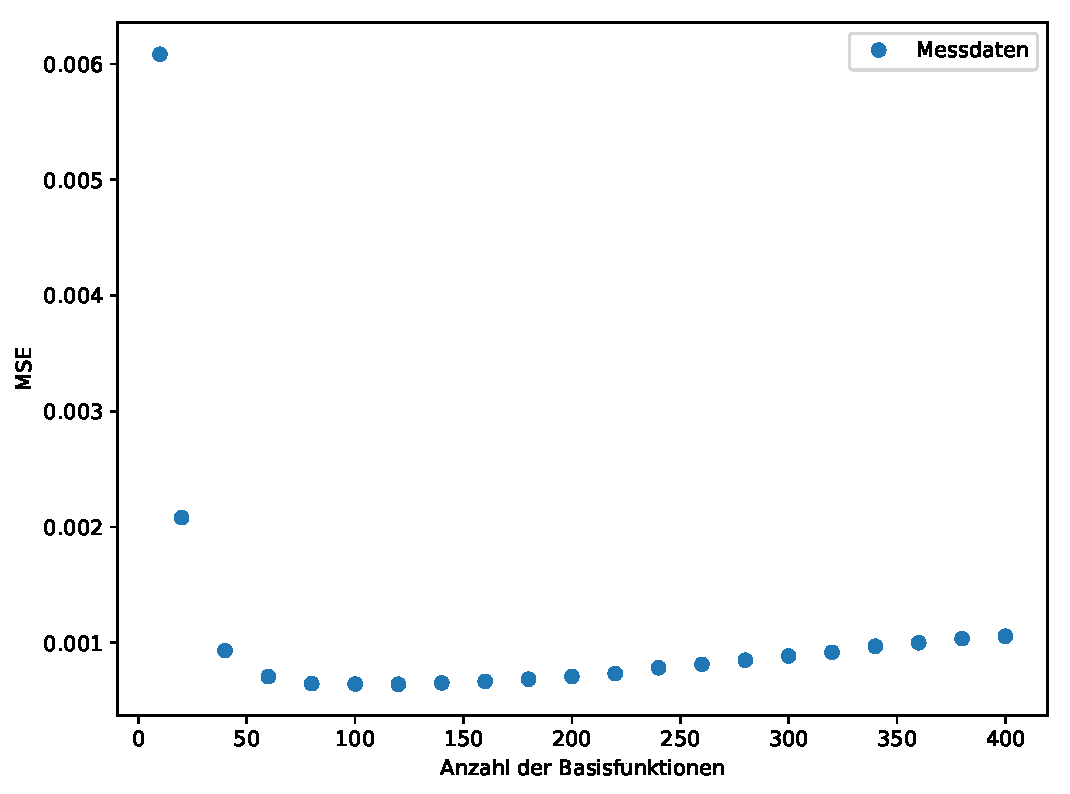
\includegraphics[width=4.2in]{figures/results/cross_prediction/rbf_placements_uv_mse.pdf}
  		\caption{Abhängigkeit des \textit{MSE}s von $l$.}
	\end{subfigure}%
	
	\caption{Darstellung der Abhängigkeit des MSE (unten) von der Anzahl der Basisfunktionen $l$ für das \textit{Barkley}-Modell\textit{Mitchell-Schaeffer}-Modell bei der Verwendung radialer Basisfunktionen.}
	\label{fig:exp_cross_rbf_placements_mse_barkley}
\end{figure}

Bei der Untersuchung des Zusammenhangs zwischen MSE und der Anzahl der Basisfunktionen kann zum einen ein asymptotischer Anteil erkannt werden, sodass der Fehler zuerst für mehr Basisfunktionen abnimmt. Allerdings lässt das Verhalten für das \textit{Mitchell-Schaeffer}-Modell erahnen, dass es hierbei einen optimalen Wert gibt, ab dem der Fehler wieder ansteigt. Dies kann durch eine schlechtere Generalisierung der Dynamik und ein zu starkes Anpassen und die Trainingsphase (auch bekannt als \textit{Overfitting}) erklärt werden. Zusammenfassend zeigt sich, dass die Wahl von $100$ Basisfunktionen eine akzeptable Abschätzung ist, sodass der Fehler möglichst gering ist und die Laufzeit auch gering gehalten wird. Diese Annahme wird im Folgenden ohne weitere qualitative Untersuchungen auf die anderen beiden Probleme übertragen, um den benötigten Rechenaufwand für die Parametersuche in einem angebrachten Rahmen zu halten.  

\FloatBarrier
\subsection{Echo State Network}
Abschließend ist dieses Problem nun mit den \textit{ESN}s gelöst worden. Dazu sind die Hyperparameter nach Abschnitt \ref{sec:exp_general_esn} gesucht worden. Die gefundenen Parameter und die damit erreichten Ergebnisse sind in Tabelle \ref{tab:exp_cross_esn_results} aufgelistet. Es ist auffällig, dass die optimalen Werte für $\sigma$ und $\Delta \sigma$ hier von denen der NN- und der RBF-Vorhersage abweichen. Auffällig ist, dass für beide Modelle die gleichen Hyperparameter die höchste Genauigkeit erzielen.\improvement{Add more details?} \\

\begin{table}[h]
	\centering
	\captionsetup{width=0.9\linewidth}
	\begin{tabular}{ccc}
		\hline		
		\multicolumn{1}{c}{} &  Barkley & Mitchell-Schaeffer \\ 
		\hline 
		\rule[-1ex]{0pt}{2.5ex} $\sigma$ & $3$ & $3$ \\ 
		\rule[-1ex]{0pt}{2.5ex} $\Delta \sigma$ & $1$ & $1$ \\ 
		\rule[-1ex]{0pt}{3.5ex} $N$ & $400$ & $400$ \\ 
		\rule[-1ex]{0pt}{3.5ex} $\rho(|\mathbf{W}|)$ & $0.95$ & $0.95$\\ 
		\rule[-1ex]{0pt}{3.5ex} $\alpha$ & $0.05$ & $0.05$ \\ 
		\rule[-1ex]{0pt}{3.5ex} $\epsilon$ & $0.1$ & $0.1$ \\ 
		\rule[-1ex]{0pt}{3.5ex} $\nu_{max}$ & $\num{1e-4}$ & $\num{1e-4}$\\ 
		\rule[-1ex]{0pt}{3.5ex} $\lambda$ & $\num{5e-6}$ & $\num{5e-6}$\\ 
		\rule[-1ex]{0pt}{2.5ex} Laufzeit [s] & $3710$ & $3733$ \\ 
		\rule[-1ex]{0pt}{2.5ex} \textbf{MSE} & \textbf{$\num{8.7e-7}$} & \textbf{0.00075} \\ 
		\rule[-1ex]{0pt}{2.5ex} \textbf{NRMSE} & \textbf{0.0039} & \textbf{0.1859} \\ 
		\hline 
	\end{tabular} 
	\caption{Ermittelte Hyperparameter des \textsc{ESN} für das \textit{Mitchell-Schaeffer}- und das \textit{Barkley}-Modell, welche zu den geringsten Fehlern führen.}
	\label{tab:exp_cross_esn_results}
\end{table}

Zuvor ist die Annahme getroffen worden, dass die Dynamik sich an jedem Punkt im Inneren des Feldes lokal ähnelt. Um diese Annahme zu untersuchen bietet es sich an die unterschiedlichen trainierten Gewichtsmatrizen $\mathbf{W_{out}}$ zu betrachten. Dies ist exemplarisch für die ermittelten Hyperparameter für das \textit{Barkley}-Modell durchgeführt und in Abbildung \ref{fig:exp_cross_esn_weights} dargestellt. Dabei gibt die vertikale Achse den Index $i$ des $i$-ten Eintrages von $\mathbf{W_{out}}$ an. Dafür sind die Matrizen $\mathbf{W_{out}} \in \mathbb{R}^{(1 + N_u + N) \times 1}$ mit $N_u = 9$ jeweils spaltenweise für $900$ Pixel in einem $30 \times 30$ Einheiten messendem Quadrat in der Mitte des Feldes aufgetragen.

\begin{figure}[H]
	\centering
	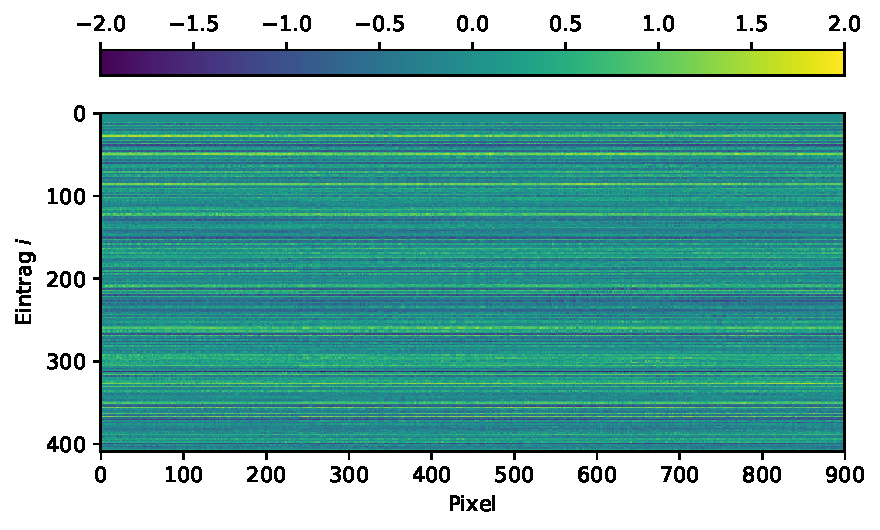
\includegraphics[height=3.0in]{figures/results/cross_prediction/weights.pdf}
	\setcapmargin[1cm]{1cm}
	\caption{Exemplarische Darstellung der Einträge der Gewichtsmatrix $\mathbf{W_{out}}$ des \textsc{ESN} für das \textit{Barkey}-Model anhand von $900$ verschiedene Bildpunkten, wobei$\mathbf{W_{out}}$ jeweils als Spalte in der Grafik dargestellt ist.}
	\label{fig:exp_cross_esn_weights}
\end{figure}

Dabei ist eine große Ähnlichkeit innerhalb der einzelnen Matrizen zu erkennen. So sind einige markante Linien in der Abbildung zu erkennen. So sind gewisse Einträge bei den Matrizen aller Pixel relativ stark beziehungsweise schwach. Trotzdem ist noch eine gewisse Varianz zuerkennen. Vermutlich wird sie dadurch verursacht, dass innerhalb der endlichen Trainingszeit nicht alle Dynamiken an jedem Pixel auftreten. Zusammenfassend kann dies als eine Bestätigung der Annahme der lokalen Ähnlichkeit gesehen werden. In weiteren Arbeiten bietet es sich an diese Frage weiter zu untersuchen und den Effekt dahingehend auszunutzen, als dass die Trainingsdaten mehrerer Punkte zusammengefasst werden können, sodass bereits aus einer kurzen Trainingszeit eine ausreichende Menge an Trainingsdaten gewonnen werden kann.
\improvement{Write something about the vanishing first 9 entries?}

\FloatBarrier
\subsection{Vergleich}
Abschließend kann nun ein Vergleich der drei verwendeten Methoden hinsichtlich ihrer Laufzeit und der erzielten Genauigkeiten durchgeführt werden. Dieser ist in Tabelle \ref{tab:exp_cross_comparison_results} zu finden. Die jeweils  besten Ergebnisse sind hervorgehoben. Die \textit{ESN}s erzielen für beide Modelle den geringsten Fehler, also die höchste Genauigkeit. Dabei ist der NRMSE für das \textit{Barkley}-Modell mehrere Größenordnung kleiner als bei den Konkurrenz-Ansätzen. Diese überaus hohe Genauigkeit ist für das \textit{Mitchell-Schaeffer}-Modell nicht erreicht worden. Hier beträgt der Fehler trotzdem etwa nur ein Drittel von dem der anderen Ansätze. Im Austausch für diese hohe Genauigkeit ist allerdings die benötigte Zeit für die Vorhersage höher als bei den Konkurrenten. Unter der Voraussetzung, dass die Rechenzeit nur eine untergeordnete Rolle spielt, so ergeben sich die \textit{ESN}s als bester Ansätze für die Kreuz-Prädiktion.
\begin{table}[h]
	\centering
	\captionsetup{width=0.9\linewidth}
	\begin{tabular}{cccccccc}
		\hline		
		\multicolumn{1}{c}{} & \multicolumn{3}{c}{Barkley} & \multicolumn{3}{c}{Mitchell-Schaeffer}		\\
		%\cline{2-7}
		\multicolumn{1}{c}{} & NN & RBF & ESN & NN & RBF & ESN \\
		
		\hline
		
		Laufzeit [s] 	& \textbf{40} 		& 1430		& 3710		& 5252		& \textbf{1434} 		& 3733 \\
		MSE 			& 0.00098	& 0.01046	& \textbf{\num{8.7e-7}} 	& 0.01891	& 0.00948 	& \textbf{0.00075} \\
		NRMSE 			& 0.1317	& 0.1023	& \textbf{\num{0.0039}} 	& 0.8795	& 0.6228 	& \textbf{0.1859} \\
		\hline 
	\end{tabular} 
	\caption{Vergleich der benötigten Laufzeit und der erreichten Fehlers der drei Ansätze für das \textit{Mitchell-Schaeffer}- und das \textit{Barkley}-Modell, welche zu den geringsten Fehlern führen.}
	\label{tab:exp_cross_comparison_results}
\end{table}

\FloatBarrier